\begin{frame}
    \frametitle{Testing}
    \centering
    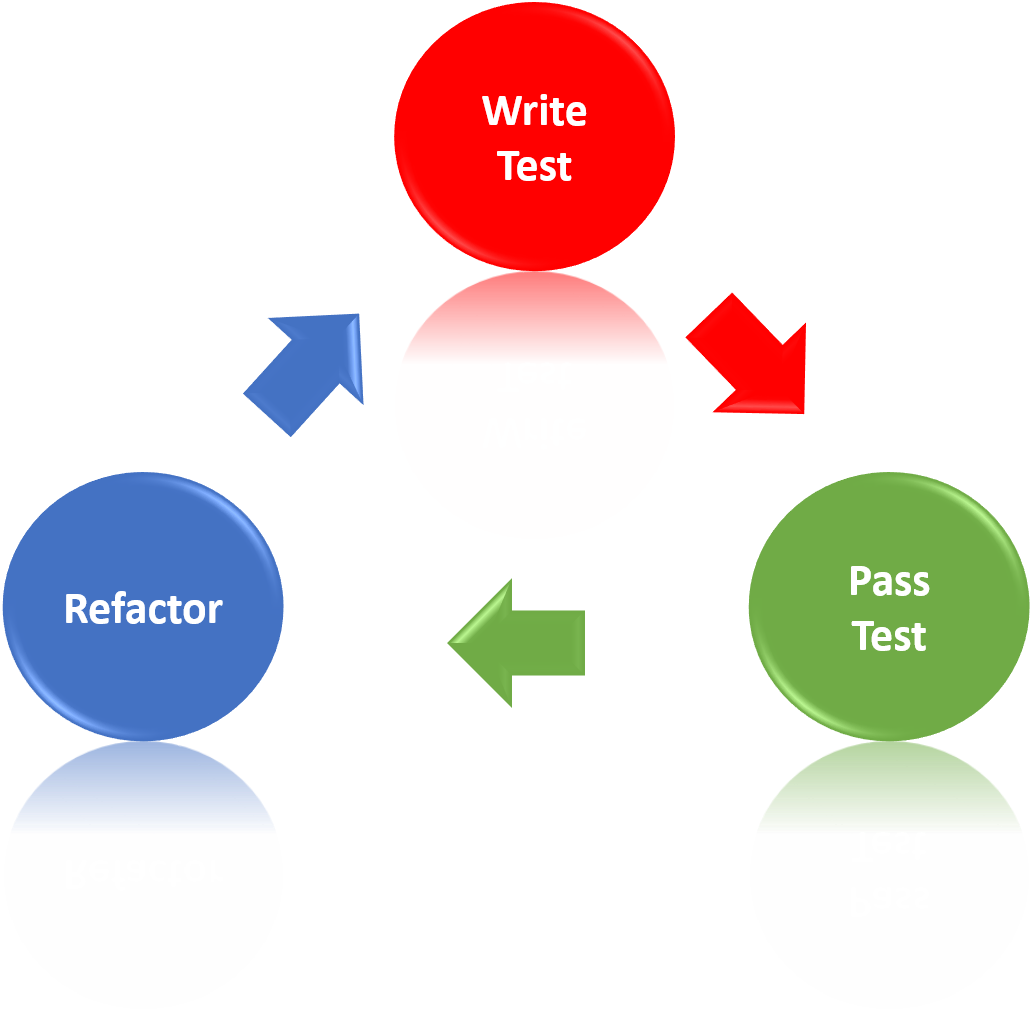
\includegraphics[scale=0.2]{Bin/testing.png}
\end{frame}


\begin{frame}
    \frametitle{Linters}
    \centering

    \textit{Linting} is the automated checking of your source code for 
    programmatic and stylistic errors without running the code
    
    \vspace{1cm}

    Linting and other tools:
    
    \begin{multicols}{3}
        \begin{itemize}
            \item black
            \item pylint
            \item flake8
            \item mccabe
            \item mypy
            \item coverage
        \end{itemize}
    \end{multicols}
\end{frame}


\begin{frame}
    \centering
    
    \color{blue}

    \textit{flake8} \\
    \vspace{0.3cm}
    \textit{pylint} \qquad \qquad \textit{mccabe} \\
    \vspace{0.2cm}

    \vspace{0.8cm}
    \textit{black} \qquad \qquad {\Huge \href{https://tox.wiki/en/latest/index.html}{\textcolor{red}{Tox}}} \qquad \qquad \textit{mypy}

    \vspace{0.8cm}
    \textit{pytest} \qquad \qquad \textit{coverage}


\end{frame}


\begin{frame}
    \frametitle{\href{https://github.com/11michalis11/AmbulanceDecisionGame/blob/master/.github/workflows/config.yml}{GitHub Actions}}
    \centering

    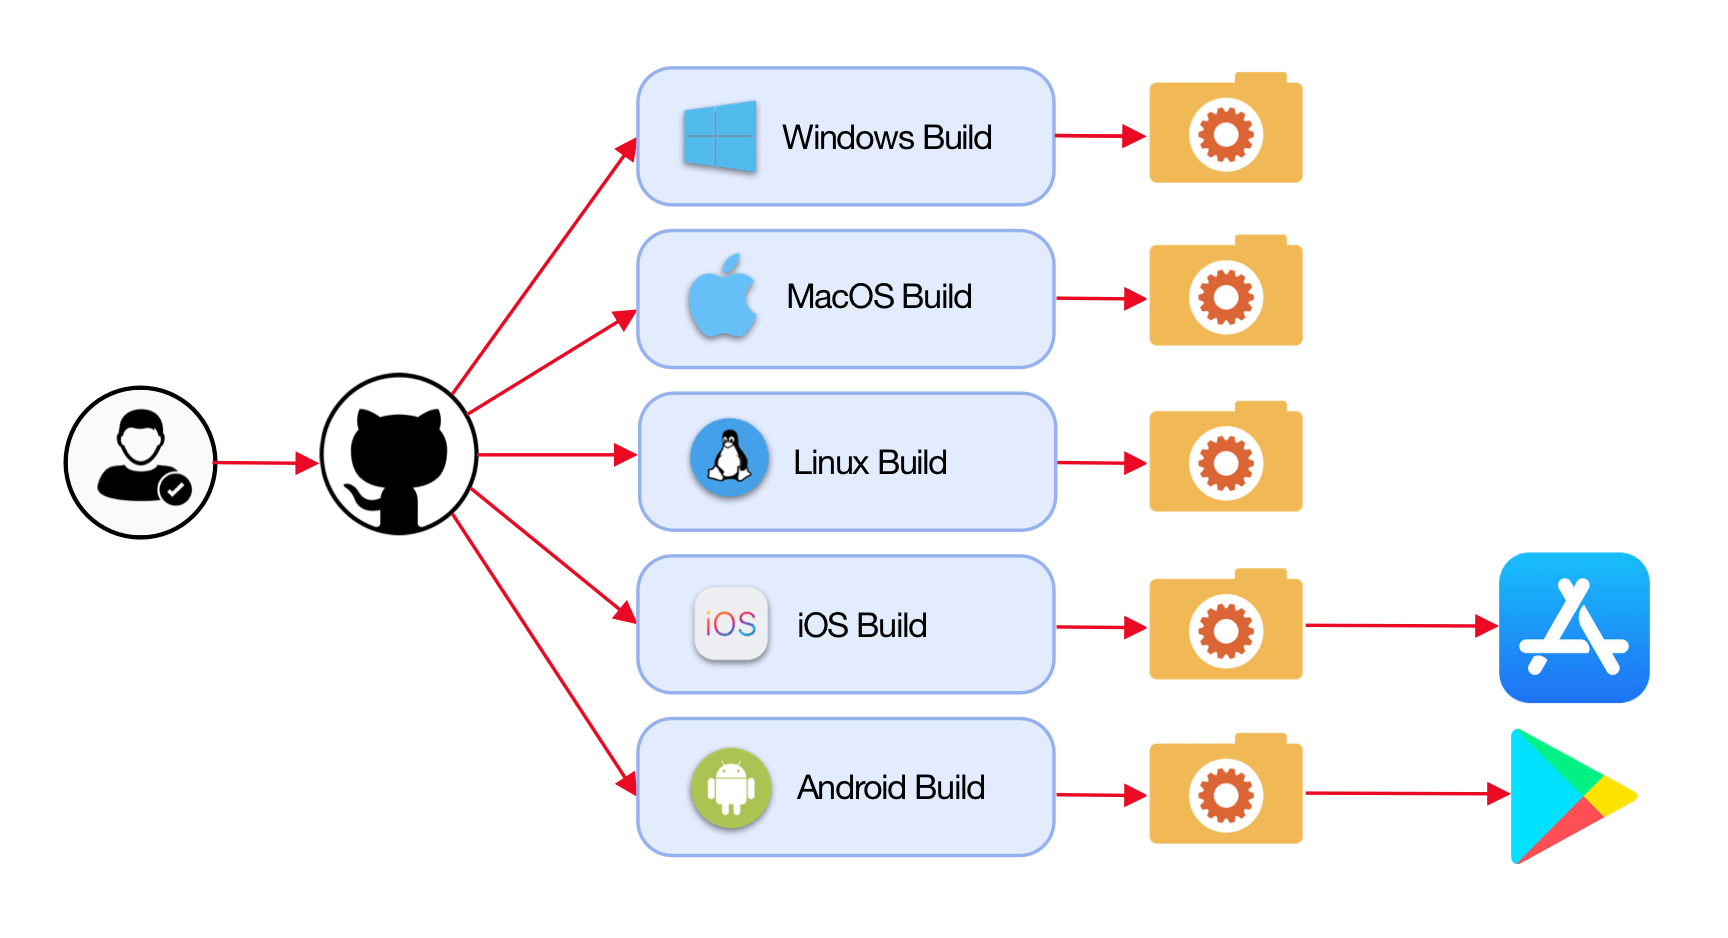
\includegraphics[width=\textwidth]{Bin/github_actions.png}

    \pause
    
    \begin{itemize}
        \item \href{https://github.com/11michalis11/ED-EMS-game-paper}{\LaTeX \(\;\) actions}
        \item \href{https://twitter.com/tartanllama/status/1163927778376462337}{Nicholas Cage action}
    \end{itemize}

\end{frame}

